% LuaLaTeX文書; 文字コードはUTF-8
\documentclass[unicode,11pt,aspectratio=169,notes]{beamer} % 'unicode'が必要
\usepackage{luatexja} % 日本語したい
\usepackage{geometry}
\usepackage{tikz}
\usepackage{pgfplots}
\usepackage{import}
\usepackage{multicol}

\DeclareMathOperator{\E}{\mathrm{E}}

\tikzset{
  heapnode/.style = {align=center, inner sep=0pt, circle, draw=yellow!80, text width=1.0em, fill=yellow},
  outside/.style = {heapnode, draw=black, fill=white},
  not_heap/.style = {heapnode, draw=blue!60, fill=blue!30}
}

\usetheme{boxes}
\usefonttheme[onlymath]{serif}

\title{精読『アルゴリズムイントロダクション 第4版』}
\subtitle{第3回}
\author{Panot}
\date{最終更新:\today}

\begin{document}

\begin{frame}
  \titlepage{}
\end{frame}

\begin{frame}{復習}
  \begin{itemize}
    \item 漸化式の解く方法色々:\textbf{置き換え法}、\textbf{再帰木法}、
    \textbf{マスター法}、\textbf{Akra-Bazzi 法}
    \item 
  \end{itemize}
\end{frame}

\begin{frame}{今日の内容}
  \begin{itemize}
    \item ヒープソート(heapsort)
    \item クイックソート(quicksort)
    \item 線形時間ソート
    \item 中央値と順序統計量
  \end{itemize}
\end{frame}

\section*{ヒープソート}

\begin{frame}
  \sectionpage{}
\end{frame}

\begin{frame}{ヒープ(heap)とは}
  \begin{itemize}
    \item weblio・研究社 新英和中辞典より「積み重ね,かたまり,山」。
    \item \textbf{二分ヒープ(binary heap)}はおおよそ完全二分木。
    \item 二種類:\textbf{max ヒープ}と\textbf{min ヒープ}。
    \item max ヒープの\textbf{ヒープ条件(heap property)}は、
    節点がその親と同等またはそれより小さい。
    \[
      A[\textsc{Parent}(i)] \geq A[i]
    \]
  \end{itemize}
  \begin{figure}
    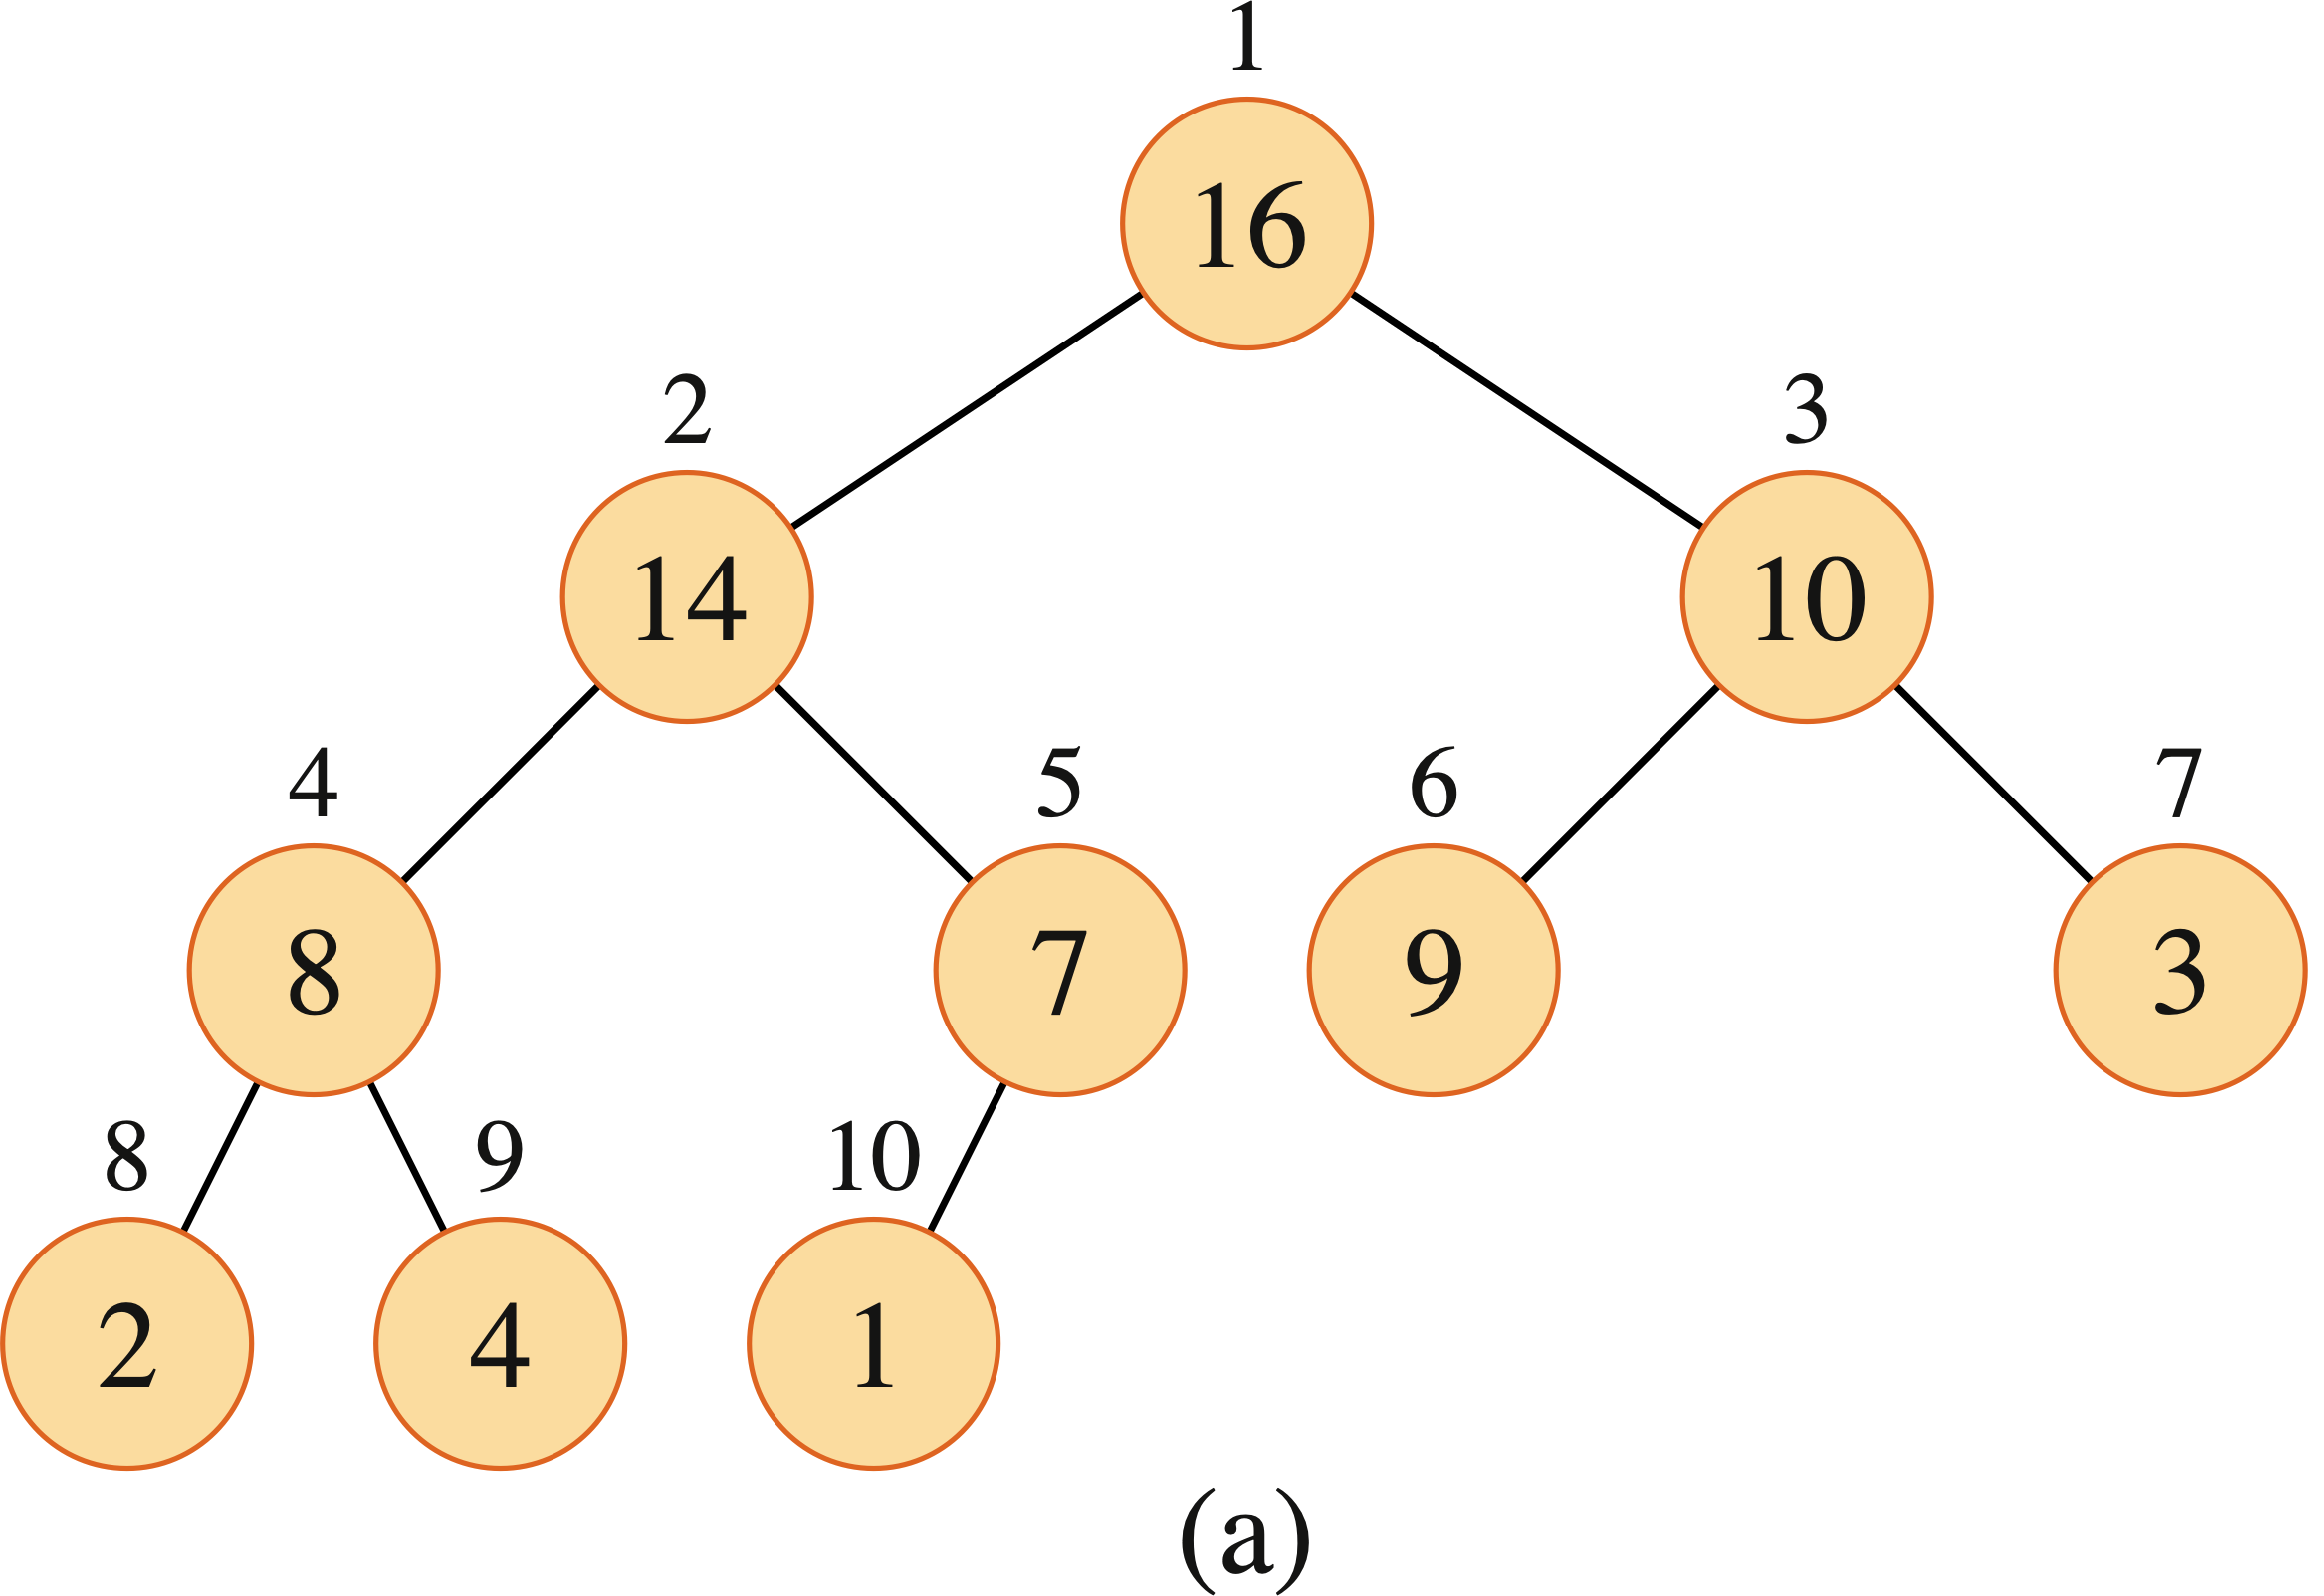
\includegraphics[height=0.4\textheight]{../resources/fig06.01a}
  \end{figure}
\end{frame}

\note[itemize]{
  \item 動的メモリ領域のことではない。
  \item 二分ではないヒープもありますが、ここでは扱いません。
  \item \textbf{おおよそ完全2分木}は、最下位階層以外すべての階層は埋まっていて、
  最下位階層では左から埋まっている。
  \item 必ず最大の値は木の根っこにある。
}

\begin{frame}{ヒープの配列による実装}
  \begin{itemize}
    \item 配列での実装は簡単。
    \item 親または子の添字は簡単に計算できる。
  \end{itemize}
  \begin{figure}
    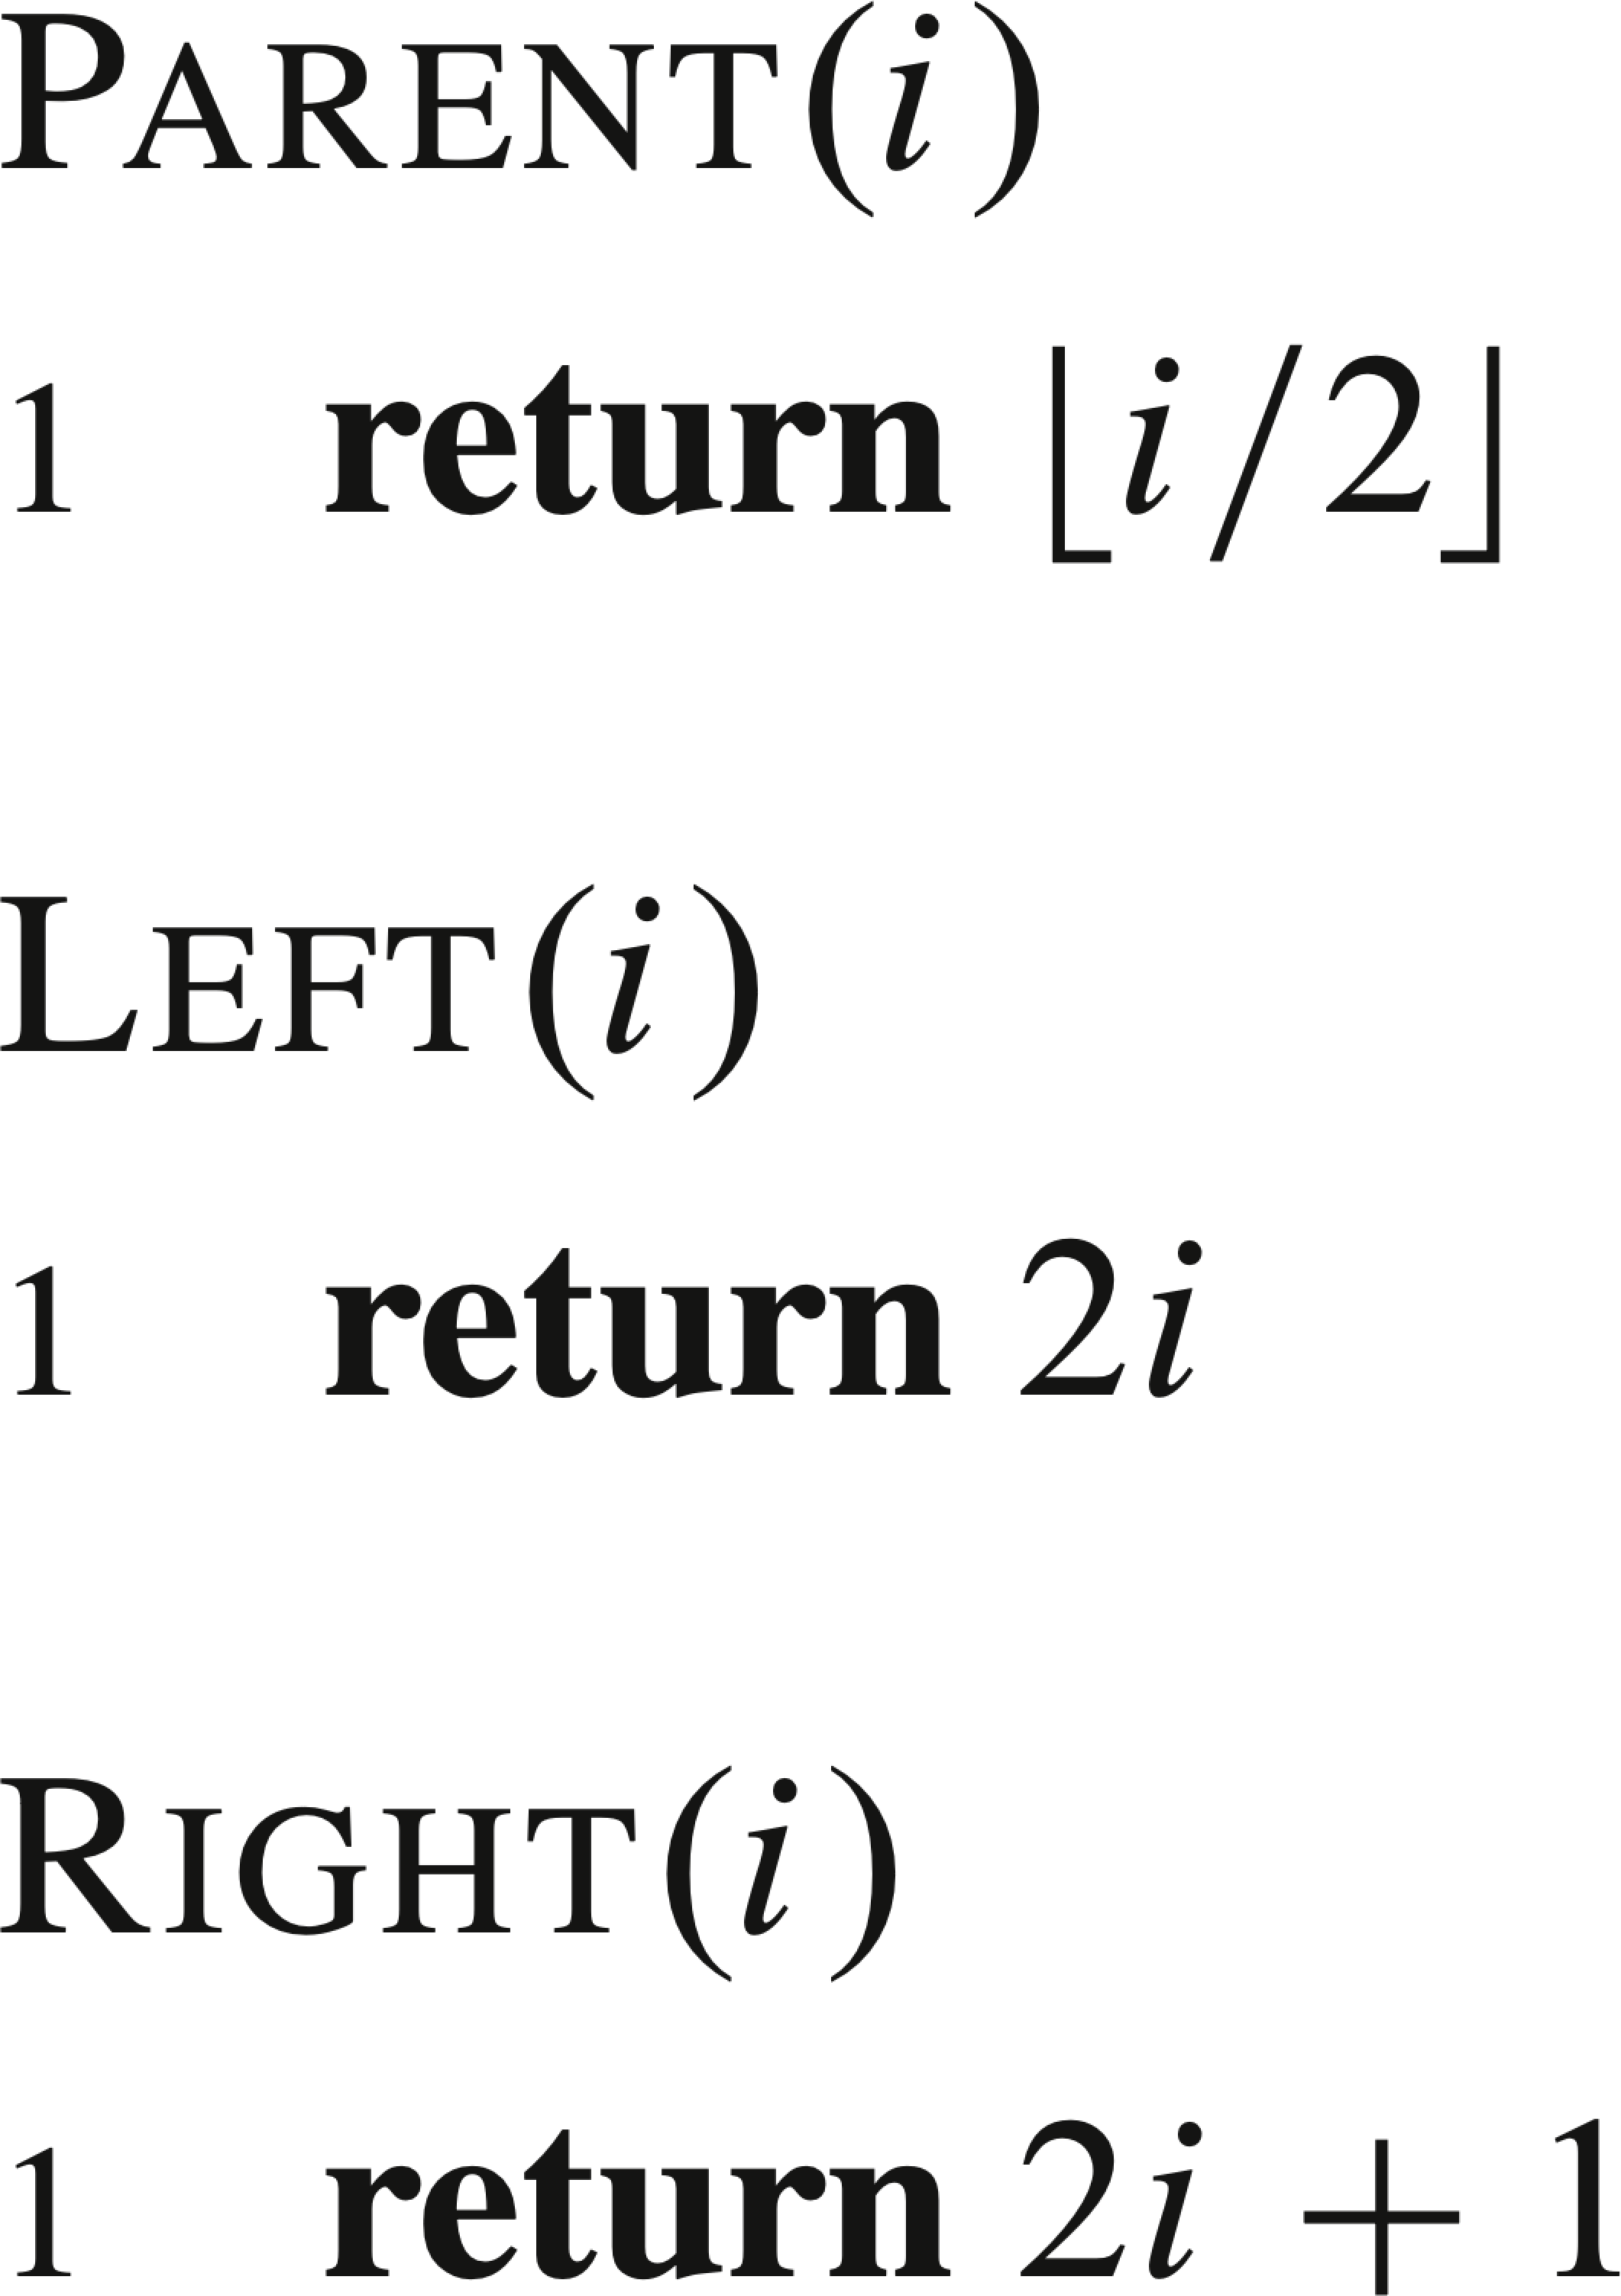
\includegraphics[height=0.4\textheight]{../resources/pseudo-06-01}
    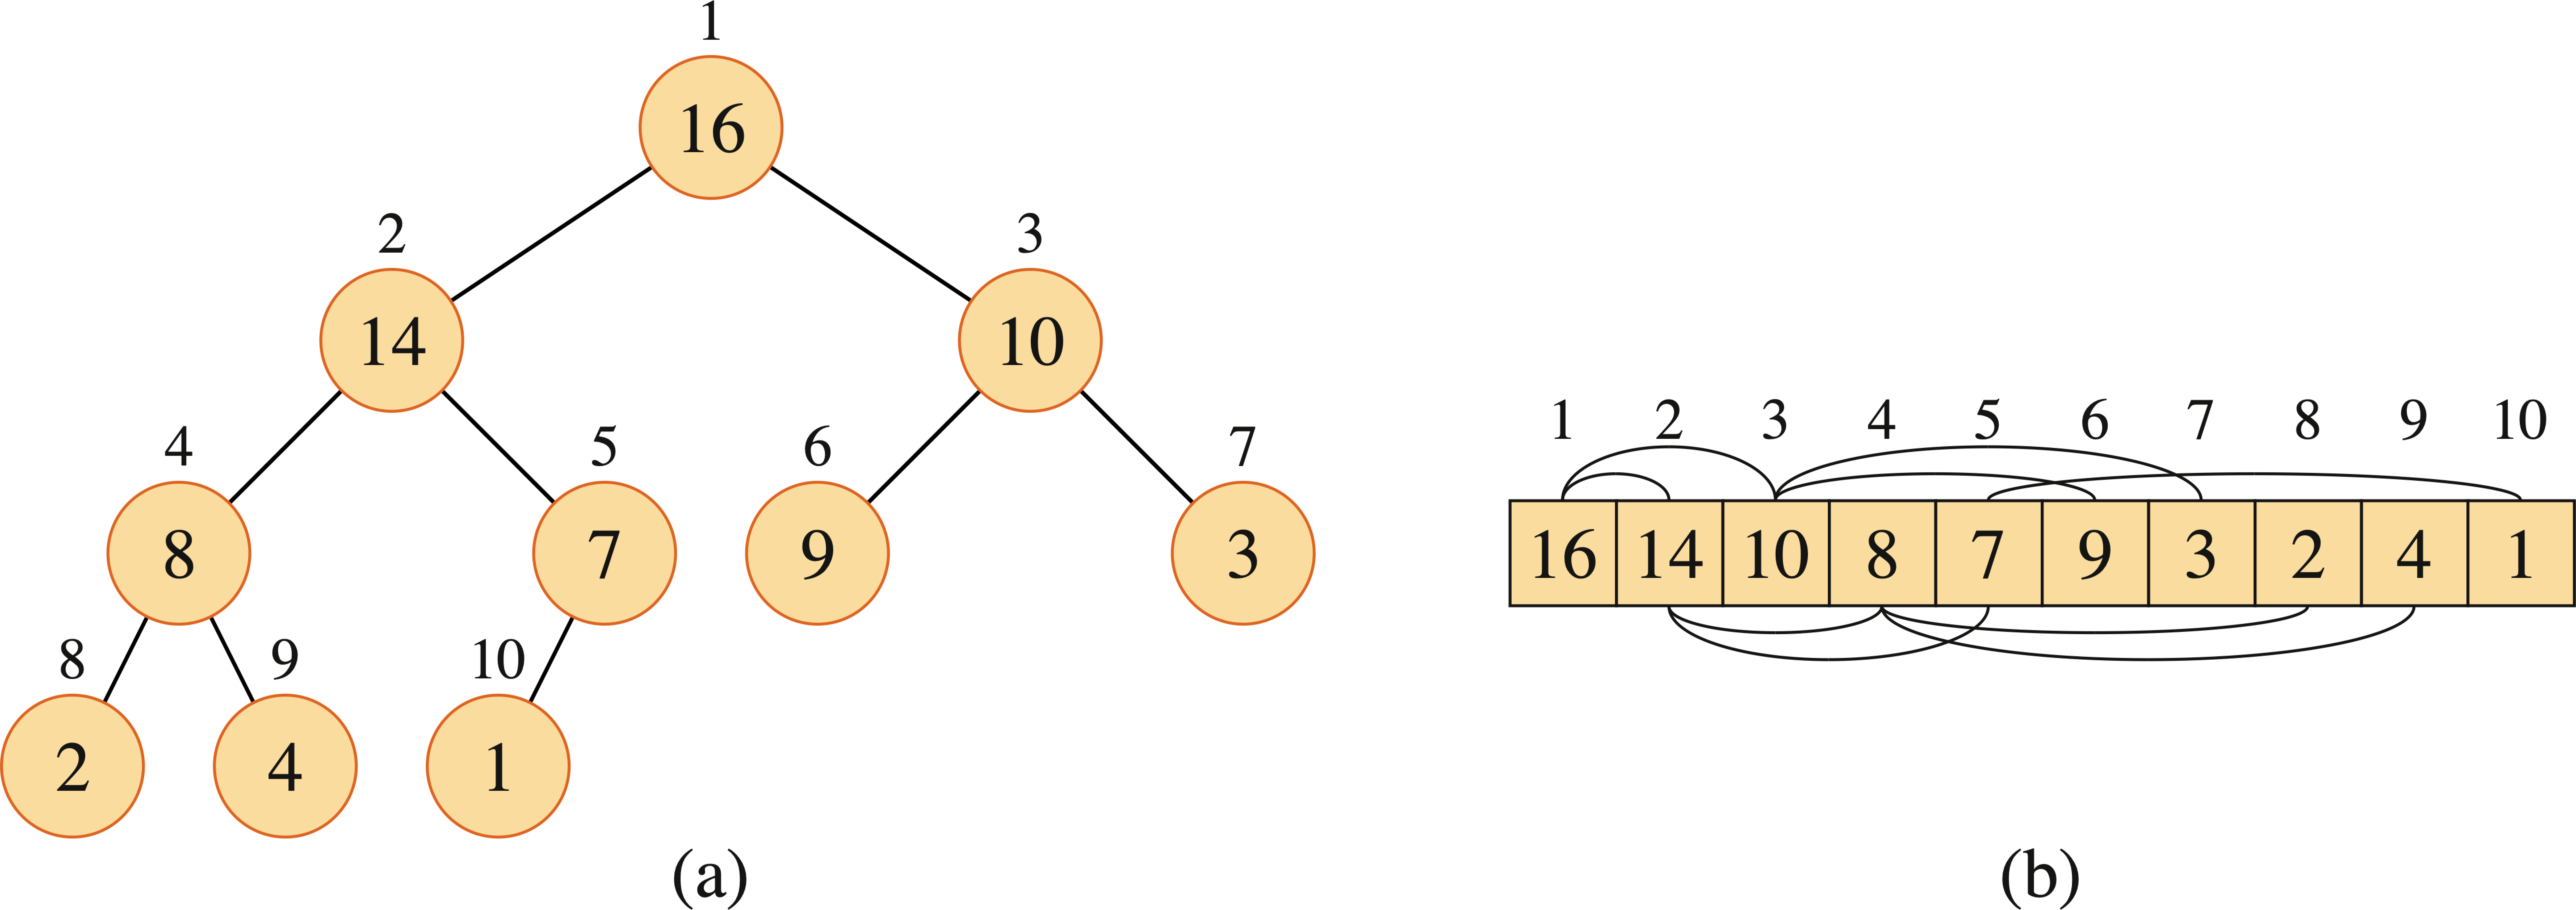
\includegraphics[height=0.4\textheight]{../resources/fig06.01}
  \end{figure}
\end{frame}

\note[itemize]{
  \item 普段の木の実装で struct を作ってポインタで参照することなど必要がない。
  \item 親または子の添字は簡単に計算できるし、配列だからメモリも線形で確保できるし、
  便利な実装です。
}

\begin{frame}[fragile]{ヒープソートの戦略}
  \begin{enumerate}
    \item 未整列の配列をヒープにする。最大要素が木の根っこにある
          \only<2->{\alert{$O(n)$}}
    \item \label{itm:heapswap} 最大要素を配列最後の要素と交換させて、
          ヒープから除外する。\only<2->{\alert{$O(1)$}}
    \item ヒープの大きさが 0 になったら停止する。
    \item \label{itm:heapprop} 全体はヒープ条件を満たさなくなったが、
    根っこの両方の子節点以下の部分木はヒープ条件を満たしたまま。
    \item 全体をヒープにする。\only<2->{\alert{$O(\lg k)$}}
    \item \ref{itm:heapswap} に戻る。
  \end{enumerate}
  \begin{figure}
    \begin{tikzpicture}[level/.style={sibling distance=2.5cm/#1, level distance=0.5cm}]
      \node [heapnode] {$16$}
        child{ node [heapnode] {$14$}
          child{ node [heapnode] {$8$}
            child{ node [heapnode] {$2$}}
            child{ node [heapnode] {$4$}}
          }
          child{ node [heapnode] {$7$}
            child{ node [heapnode] {$1$}}
            child{ edge from parent[draw=none]}
          }
        }
        child{ node [heapnode] {$10$}
        child{ node [heapnode] {$9$}}
        child{ node [heapnode] {$3$}}};
    \end{tikzpicture}
    \begin{tikzpicture}[level/.style={sibling distance=2.5cm/#1, level distance=0.5cm}]
      \node [not_heap] {$1$}
        child{ node [heapnode] {$14$}
          child{ node [heapnode] {$8$}
            child{ node [heapnode] {$2$}}
            child{ node [heapnode] {$4$}}
          }
          child{ node [heapnode] {$7$}
            child{ node [outside] {$16$} edge from parent[draw=none]}
            child{ edge from parent[draw=none]}
          }
        }
        child{ node [heapnode] {$10$}
        child{ node [heapnode] {$9$}}
        child{ node [heapnode] {$3$}}};
    \end{tikzpicture}
    \begin{tikzpicture}[level/.style={sibling distance=2.5cm/#1, level distance=0.5cm}]
      \node [heapnode] {$14$}
        child{ node [heapnode] {$8$}
          child{ node [heapnode] {$4$}
            child{ node [heapnode] {$2$}}
            child{ node [heapnode] {$1$}}
          }
          child{ node [heapnode] {$7$}
            child{ node [outside] {$16$} edge from parent[draw=none]}
            child{ edge from parent[draw=none]}
          }
        }
        child{ node [heapnode] {$10$}
        child{ node [heapnode] {$9$}}
        child{ node [heapnode] {$3$}}};
    \end{tikzpicture}
  \end{figure}
\end{frame}

\note[itemize]{
  \item おおまかに見れば、最大要素を1個ずつ探していくように見える。
  \item 単純にそれだけだと、\textbf{選択ソート}と同じで、実行時間は $O(n^2)$ になる。
  \item 無秩序に残っている要素の中で最大要素を探し出すのは、
  残っている要素の数 $n$ に対して実行時間 $O(n)$ であるため、
  全体の実行時間は $O(n^2)$ になる。これはためだ。
  \item ヒープソートのキモはヒープの性質。
  \ref{itm:heapprop} に書いてあるように、最大要素を別の要素と交換しても、
  それ以下両方の部分木はヒープ条件を満たしているままということ。
  \item その性質のもとで、全体がヒープ条件を満たすようにするのは $O(\lg n)$
  の実行時間しか要しないため、選択ソートより速い。
}

\begin{frame}[label=figheapsort]{ヒープソートの実行例}
  \begin{figure}
    \includegraphics[height=0.9\textheight]{../resources/fig06.04}
  \end{figure}
\end{frame}

\begin{frame}{必要な手続き}
    \begin{itemize}
      \item 両方の部分木がヒープ条件を満たしたとき、全体をヒープにする。
            \only<2->{\alert{\textsc{Max-Heapify} $O(\lg n)$}}
      \item 未整列の配列をヒープにする。
            \only<2->{\alert{\textsc{Build-Max-Heap} $O(n)$}}
      \item ヒープソート。
            \only<2->{\alert{\textsc{Heapsort} $O(n\lg n)$}}
  \end{itemize}
\end{frame}

\note[itemize]{
  \item \textsc{Max-Heapify} を先に紹介するのは \textsc{Build-Max-Heap} がそれを
  利用するためです。
}

\begin{frame}{\textsc{Max-Heapify}}
  \begin{itemize}
    \item 両方の部分木がヒープ条件を満たしている。
    \item 根っこがその子より小さかったら3つの中の最大の要素を根っこと交換する。
    \item 交換した部分木を \textsc{Max-Heapify} を適用する。
    \item \alert{$O(\lg n)$}
  \end{itemize}
  \only<1>{
  \begin{figure}
    \includegraphics[height=0.6\textheight]{../resources/fig06.02}
  \end{figure}
  }
  \only<2>{
  \begin{figure}
    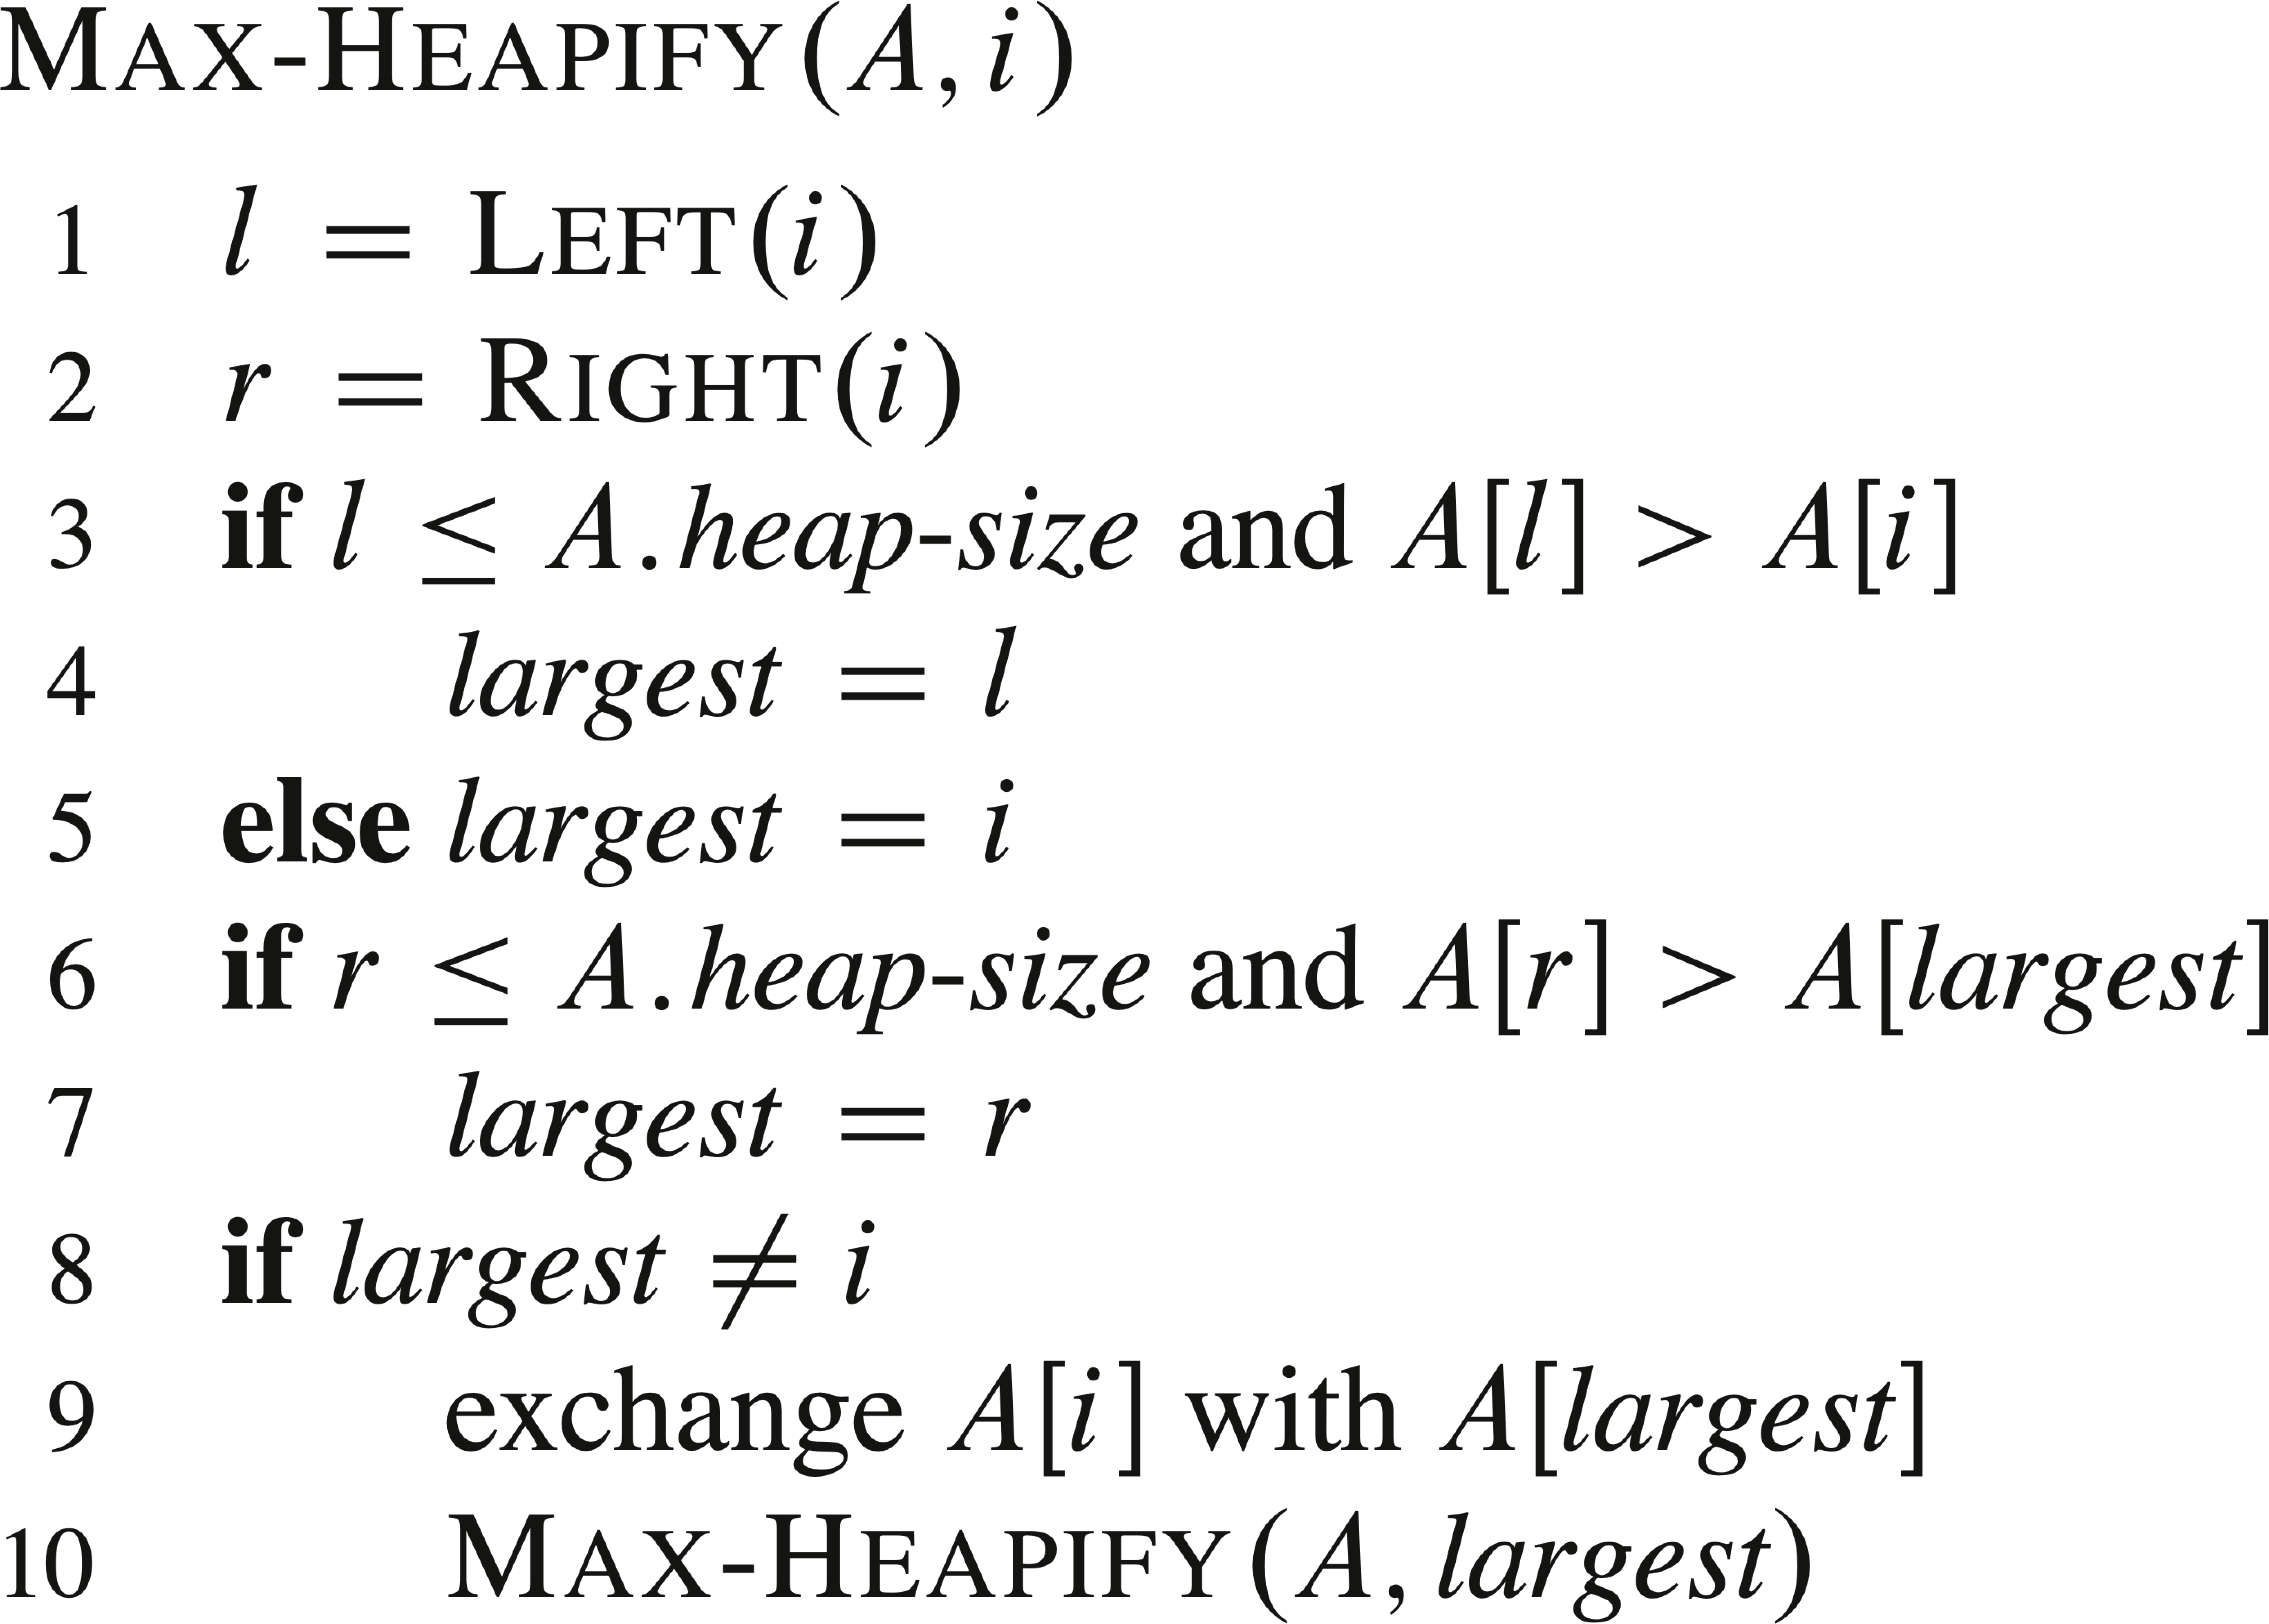
\includegraphics[height=0.6\textheight]{../resources/pseudo-06-02}
  \end{figure}
  }
\end{frame}

\note[itemize]{
  \item 根っこを適当なところまで沈める。
}

\begin{frame}{\textsc{Build-Max-Heap}}
  下からヒープを作る。\only<2>{$O(n \lg n)$ だが、\alert{$O(\lg n)$}でもある!}
  \only<1>{
  \begin{figure}
    \includegraphics[height=0.8\textheight]{../resources/fig06.03}
  \end{figure}
  }
  \only<2>{
  \begin{figure}
    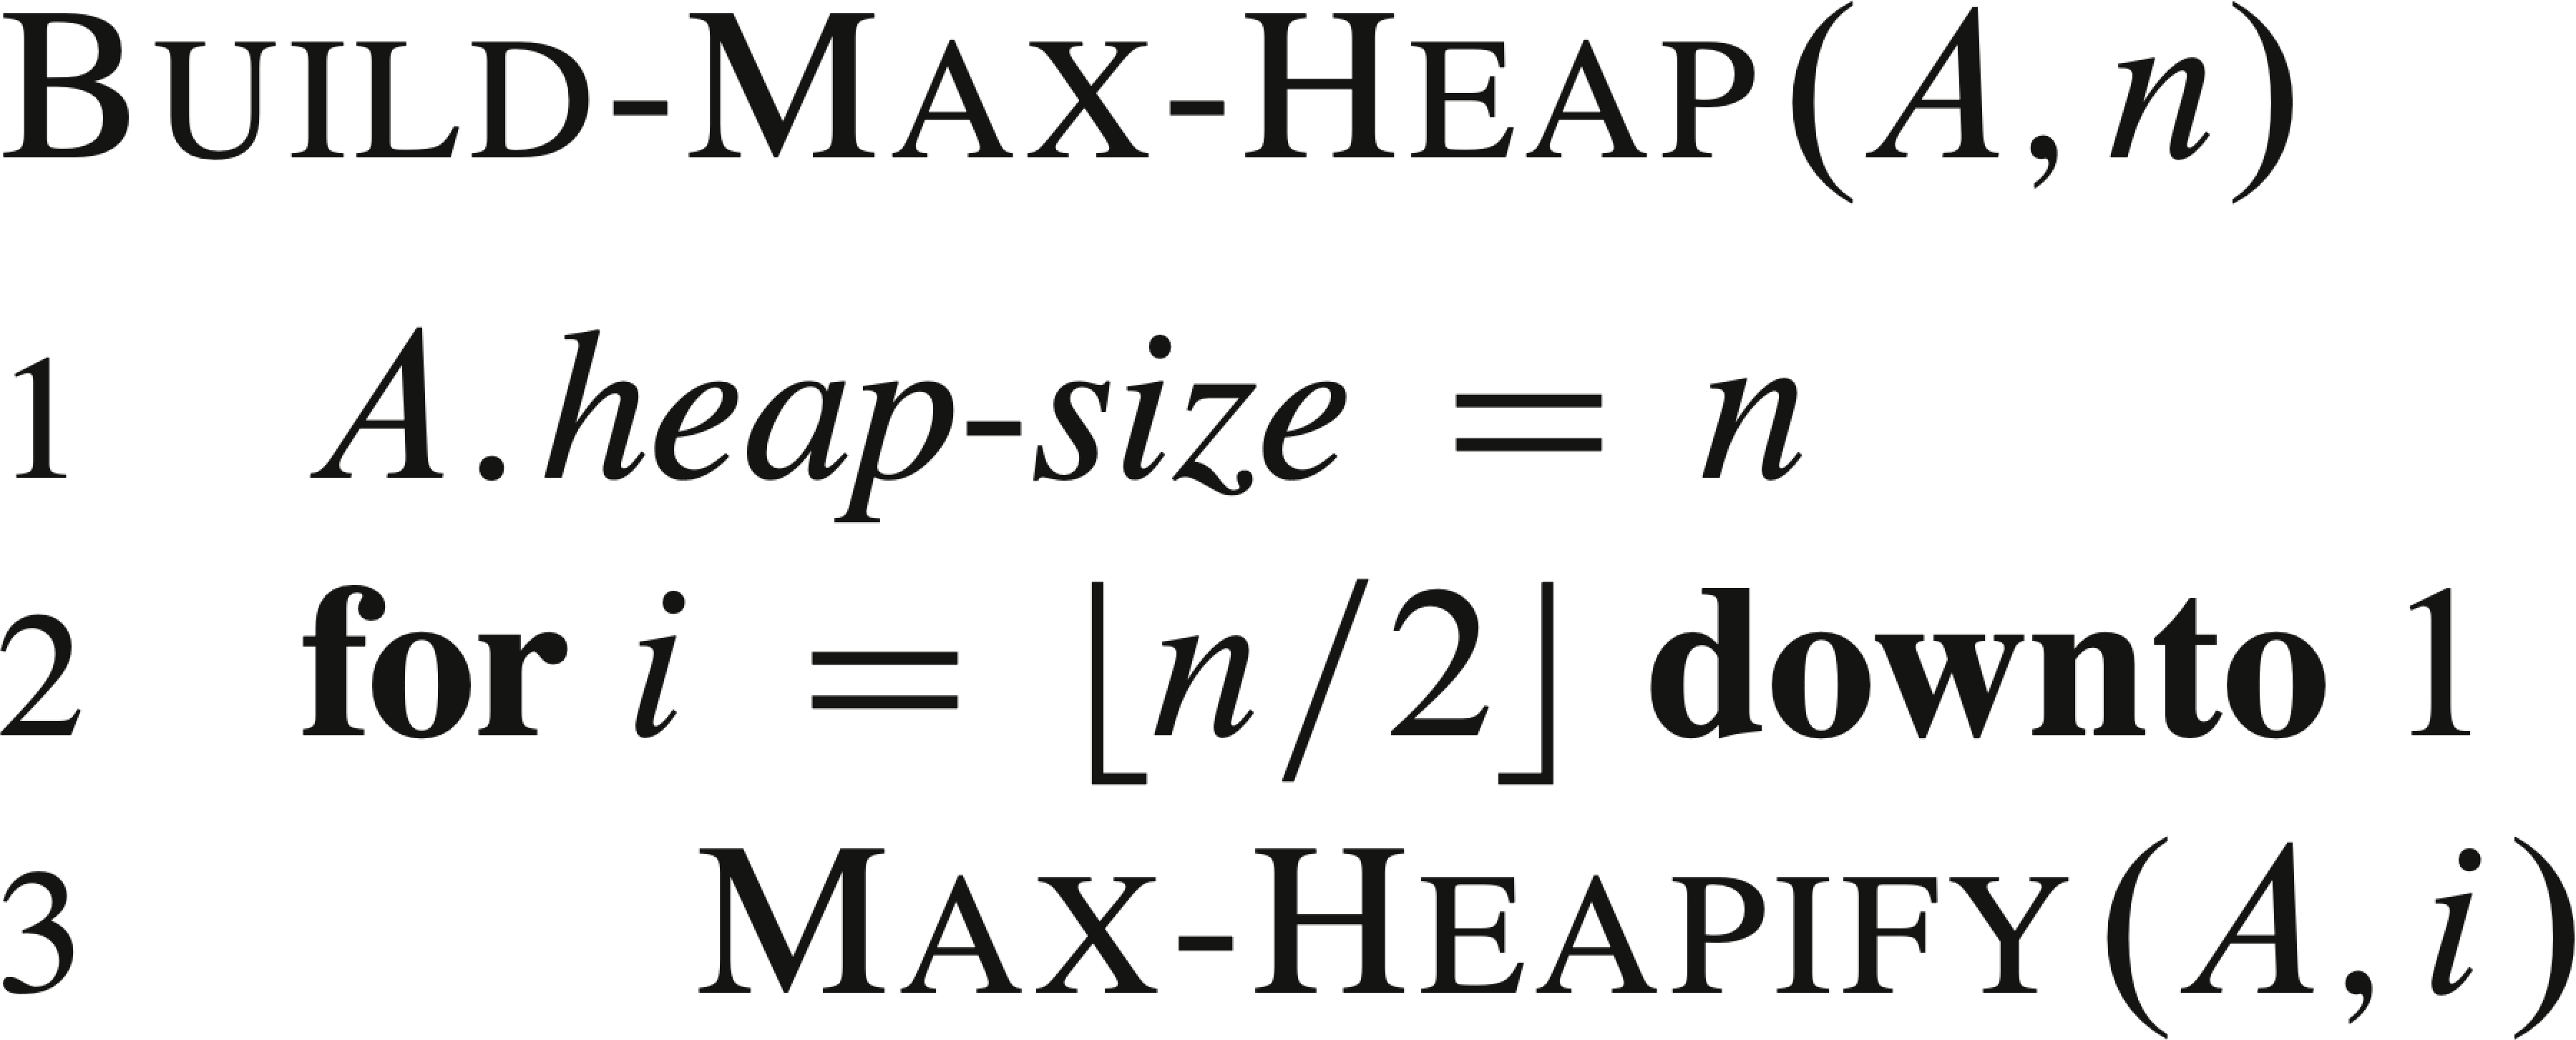
\includegraphics[width=0.6\textwidth]{../resources/pseudo-06-03}
  \end{figure}
  }
\end{frame}

\note[itemize]{
  \item 未整列の配列を二分木とみなす。
  \item 葉っぱは既にヒープである。
  \item \textsc{Max-Heapify} を使って、下から全体をヒープにしていく。
}

\begin{frame}{ヒープソート}
  \begin{enumerate}
    \item 未整列の配列をヒープにする。最大要素が木の根っこにある
          \alert{$O(n)$}
    \item \label{itm:heapswap} 最大要素を配列最後の要素と交換させて、
          ヒープから除外する。\alert{$O(1)$}
    \item ヒープの大きさが 0 になったら停止する。
    \item \label{itm:heapprop} 全体はヒープ条件を満たさなくなったが、
          根っこの両方の子節点以下の部分木はヒープ条件を満たしたまま。
    \item 全体をヒープにする。\alert{$O(\lg k)$}
    \item \ref{itm:heapswap} に戻る。
  \end{enumerate}
  \only<2->{
  \begin{figure}
    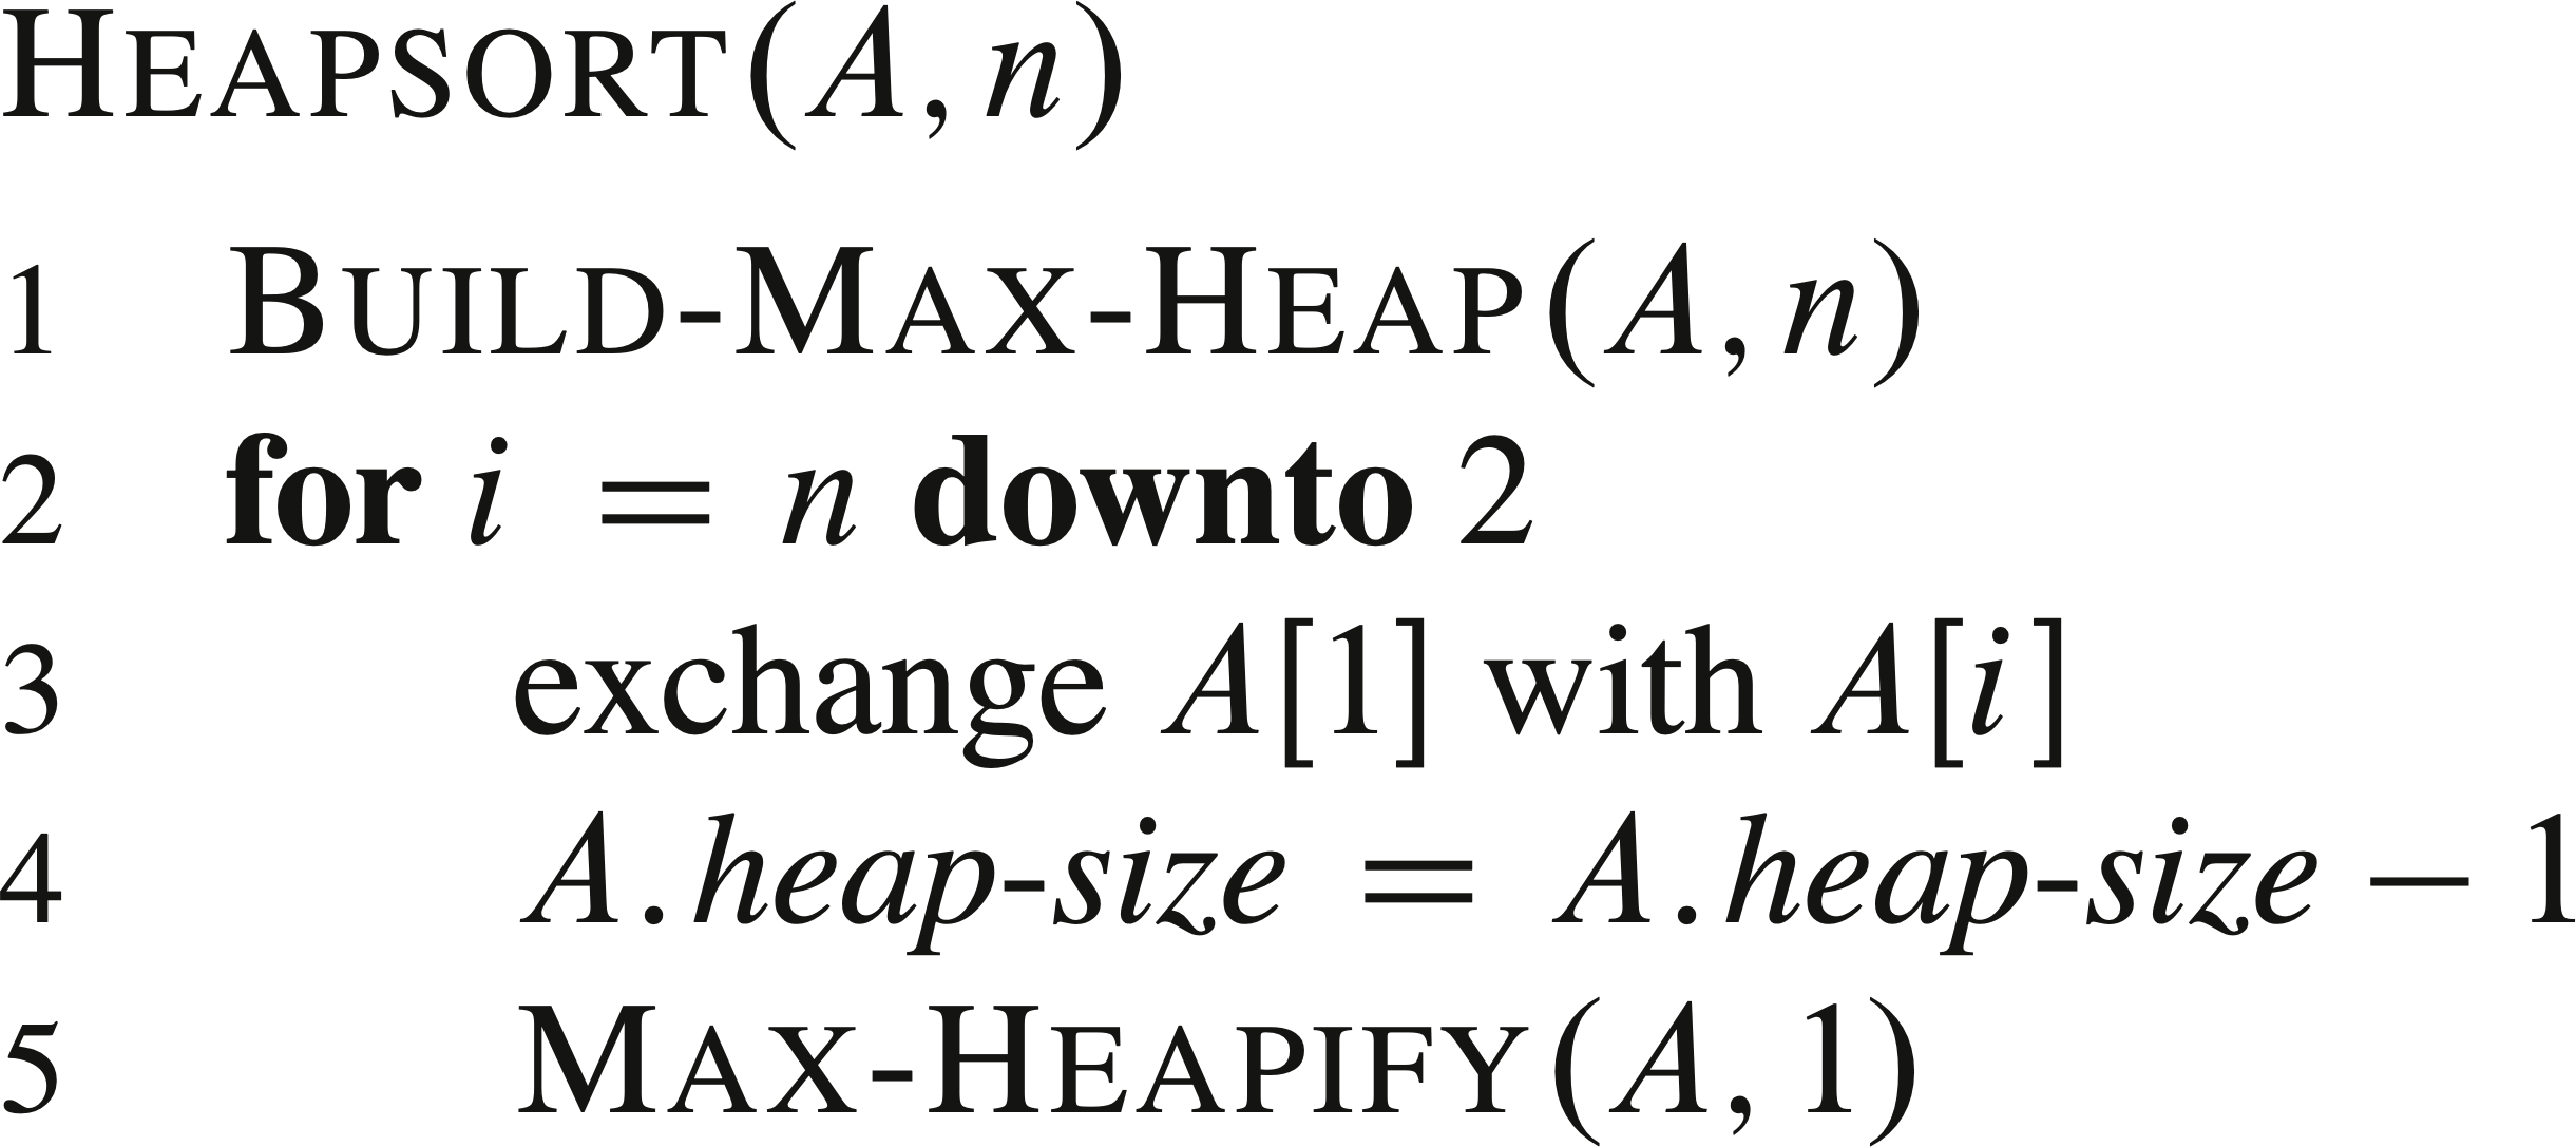
\includegraphics[height=0.3\textheight]{../resources/pseudo-06-04}
  \end{figure}
  }
  \only<3>{ヒープソートは \alert{$O(n \lg n)$}}
\end{frame}

\againframe{figheapsort}

\begin{frame}{優先度付きキュー(priority queue)}
  \begin{itemize}
    \item \textbf{優先度付きキュー(priority queue)}は、
          各要素に優先度がついている要素の集合。
    \item \textbf{max 優先度付きキュー}は、この集合から常に
          優先度が最大のものを取り出す操作が用意されているもの。
    \item 次の操作が用意されている:
      \begin{itemize}
        \item \textsc{Insert} 挿入
        \item \textsc{Maximum} 優先度が最大の要素を返す
        \item \textsc{Extract-Maximum} 優先度が最大の要素を取り出す
        \item \textsc{Increase-Key} キュー内の要素の優先度を上げる
      \end{itemize}
  \end{itemize}
\end{frame}

\note[itemize]{
  \item max 優先度付きキューに対して min 優先度付きキューもある。
  \item タスクがいっぱいあるときに、一番重要なものを先に実行するようなイメージ。
  \item 配列でも実装できるが、実行時間が長いです。整列させて、順番に取り出したらいい
}

\begin{frame}<1>[label=priority-compare]{実装の比較}
  \begin{table}
    \begin{tabular}{|c|c|c|c|c|}
      \hline
      実装 & 初期化 & 取り出し & 挿入 & 優先度変更 \\
      \hline
      整列された配列 & $O(n \lg n)$ & $O(1)$ & $O(n)$ & $O(n)$ \\
      ヒープ & $O(n \lg n)$ & \only<2->{\alert<2>{$O(\lg n)$}} &
      \only<3->{\alert<3>{$O(\lg n)$}} &
      \only<3->{\alert<3>{$O(\lg n)$}} \\
      \hline
    \end{tabular}
  \end{table}
\end{frame}

\begin{frame}{\textsc{Maximum} と \textsc{Extract-Maximum}}
  \begin{itemize}
    \item<+-> 優先度が最大の要素を返す操作は \alert{$O(1)$}。
    \item<+-> 優先度が最大の要素を取り出す操作は:
    その要素をヒープから除外して、集合をまたヒープにする。 \alert{$O(\lg n)$}。
  \end{itemize}
  \only<+->{
  \begin{figure}
    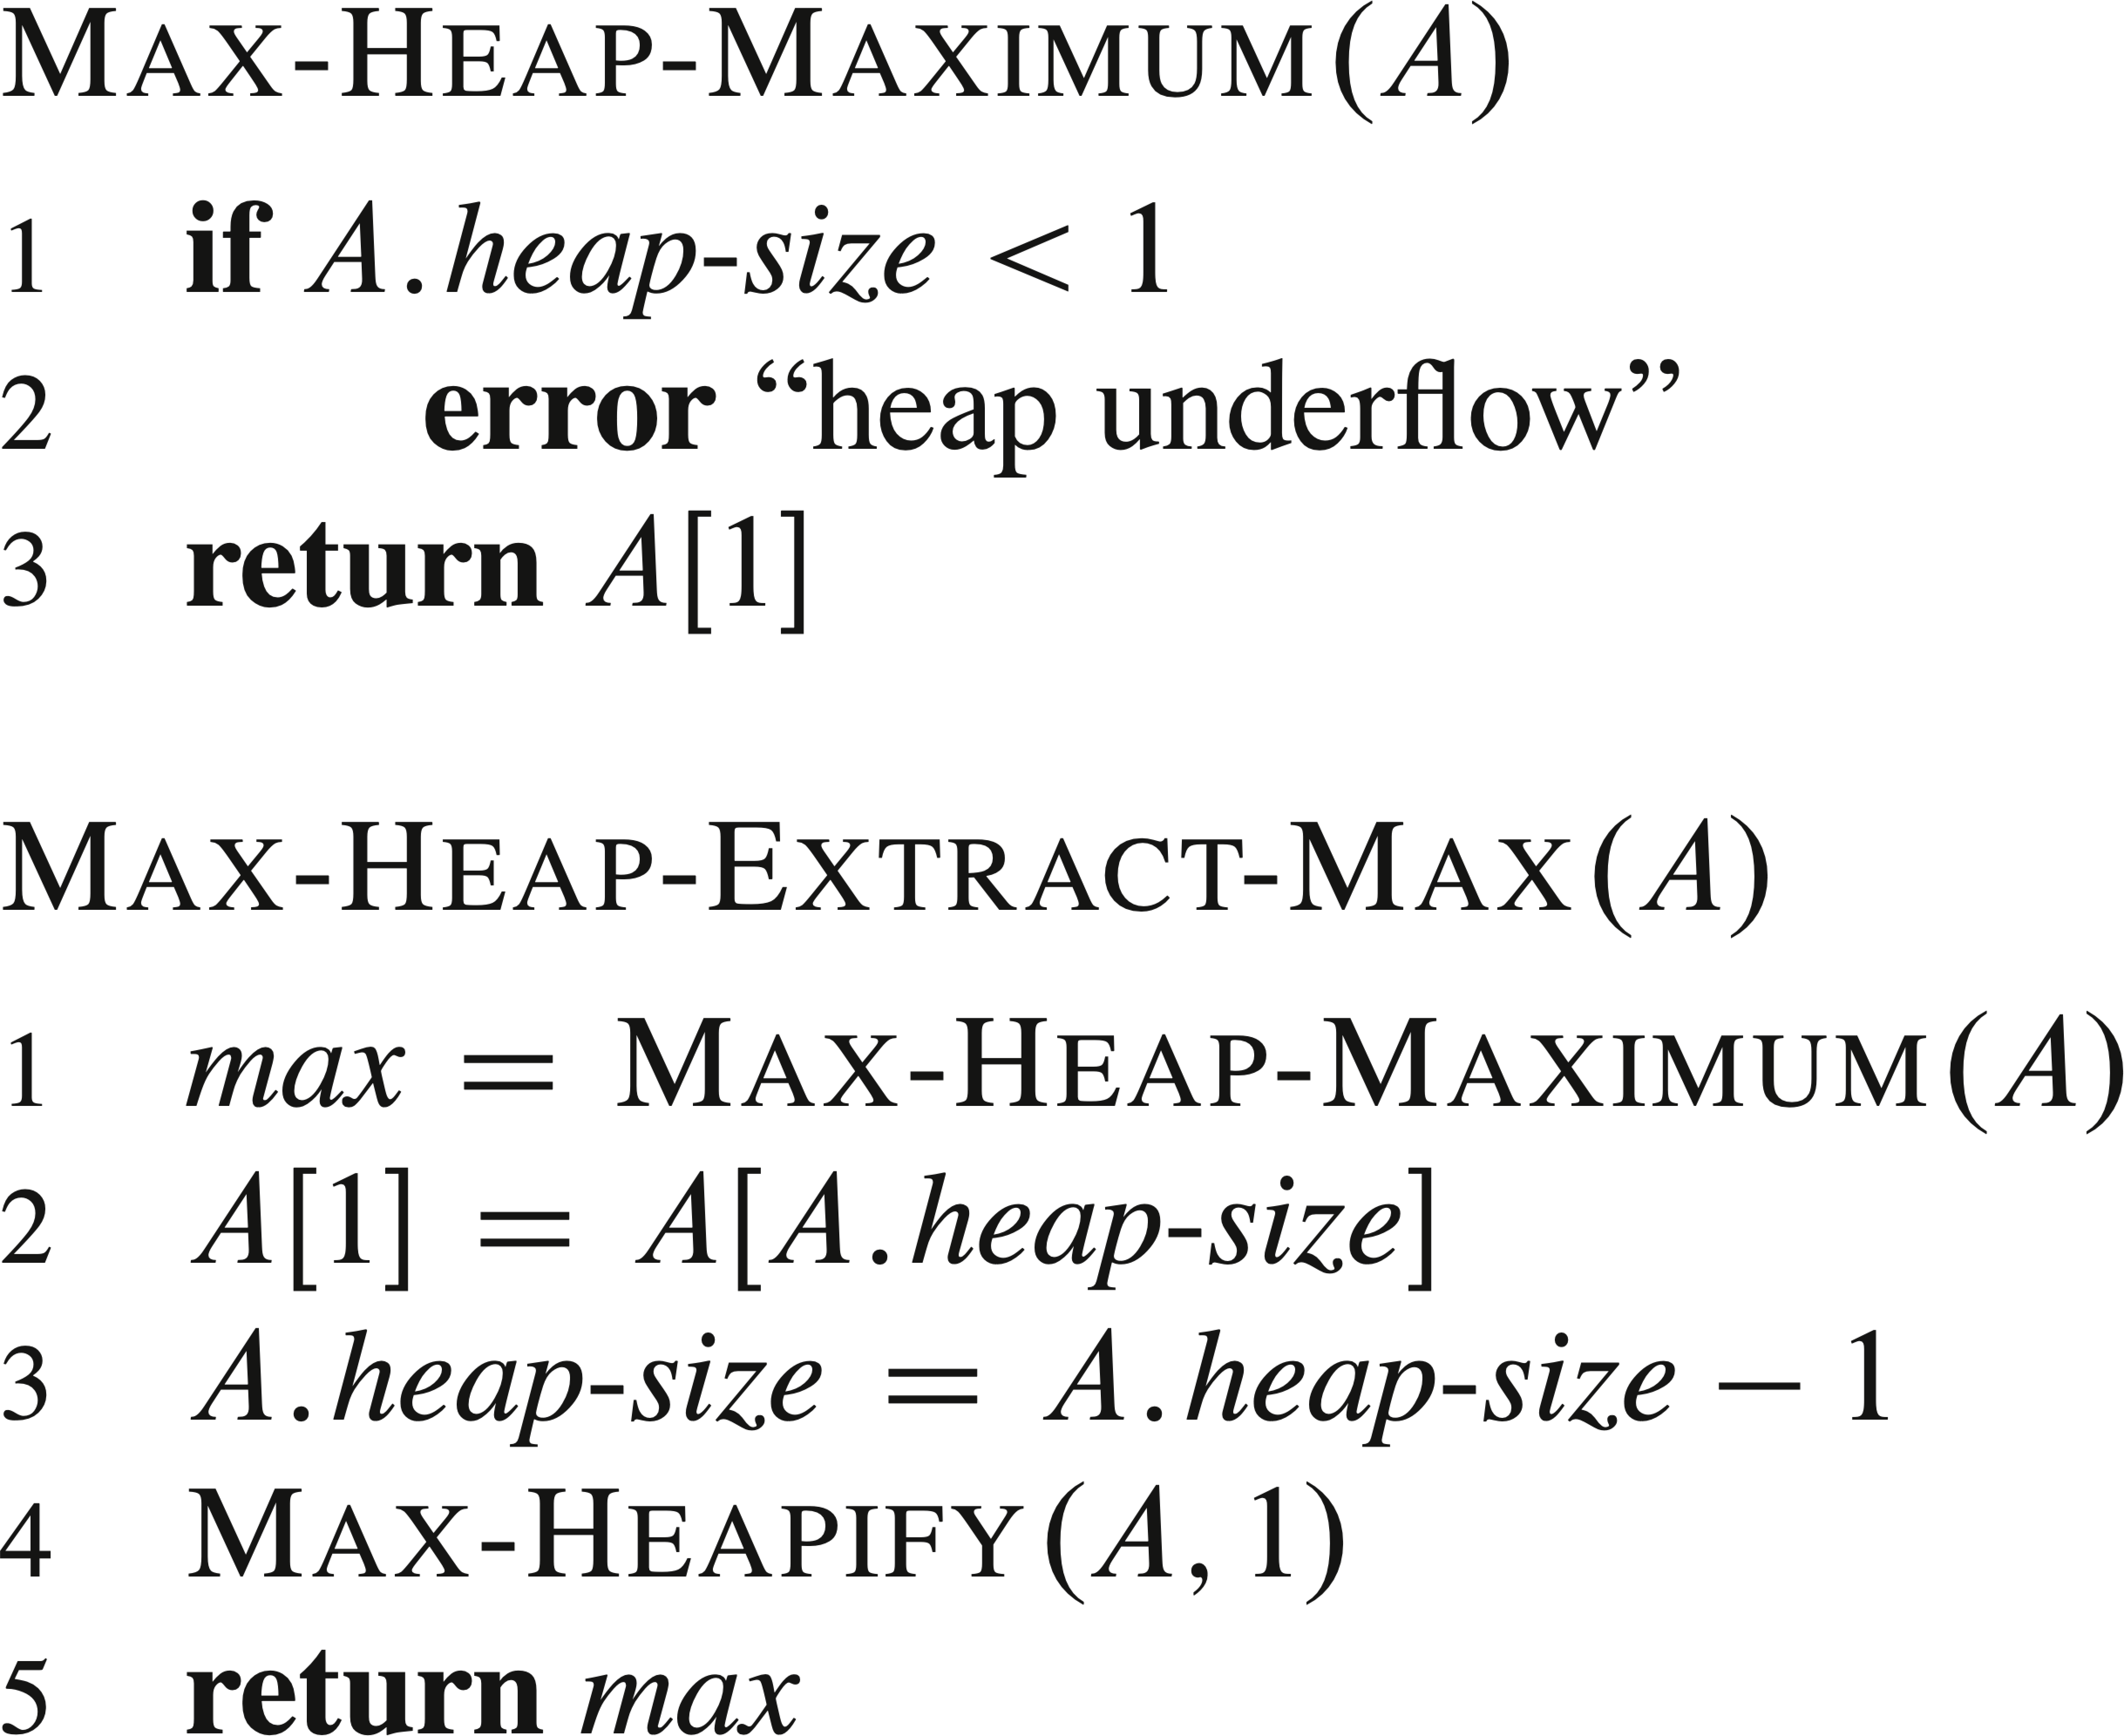
\includegraphics[height=0.5\textheight]{../resources/pseudo-06-05}
  \end{figure}
  }
\end{frame}

\note[itemize]{
  \item 返すは根っこを参照するだけで十分。
  \item 取り出す操作は、参照して、集合から除外して、残りをまらヒープにする。
  ヒープソートのループ内と同じ操作。
  \item ここまではヒープソートと同じ。
}

\againframe<2>{priority-compare}

\begin{frame}{\textsc{Increase-Key} と \textsc{Insert}}
  \begin{itemize}
    \item キュー内の要素の優先度を上げる。
    \item 優先度を上げても、その要素を根っことした部分木はまだヒープ。
    \item ただし、その親以上の部分木はヒープと限らない。
    \item 親より優先度が大きかったら交換していく。
  \end{itemize}
  \only<+->{
  \begin{figure}
    \includegraphics[height=0.5\textheight]{../resources/fig06.05}
  \end{figure}
  }
  \only<+->{
    挿入も、とりあえず葉っぱにくっつけて浮上させる。
  }
\end{frame}

\note[itemize]{
  \item その要素を適当なところまで浮上させる。
  \item \textsc{Max-Heapify} と逆の操作。
}

\begin{frame}{\textsc{Increase-Key} と \textsc{Insert}}
  \begin{figure}
    \includegraphics[height=0.8\textheight]{../resources/pseudo-06-06}
  \end{figure}
\end{frame}

\againframe<3>{priority-compare}

\end{document}
